\documentclass[10pt,letterpaper, onecolumn]{report}
\usepackage{amsmath}
\usepackage{amssymb}
\usepackage{listings}
\usepackage{xcolor}
\usepackage[lmargin=71pt, tmargin=0.6in]{geometry}
\usepackage{fancyhdr}
\usepackage{graphicx}

% Footer format
\pagestyle{fancy}
\fancyhead{}
\fancyfoot{}
\fancyfoot[L]{Author: Kacper Ragankiewicz, Index: 283415}
\fancyfoot[R]{\thepage}

% Syntax highlighting for Python
\definecolor{keywordcolor}{rgb}{0.58, 0.01, 0.24}
\definecolor{stringcolor}{rgb}{0.44, 0.55, 0.34}
\definecolor{commentcolor}{rgb}{0.5, 0.5, 0.5}
\definecolor{backgroundcolor}{rgb}{0.97, 0.97, 0.97}

\lstdefinestyle{myPythonStyle}{
    language=Python,
    backgroundcolor=\color{backgroundcolor},
    basicstyle=\ttfamily\small,
    keywordstyle=\color{keywordcolor}\bfseries,
    stringstyle=\color{stringcolor},
    commentstyle=\color{commentcolor}\itshape,
    numberstyle=\tiny\color{gray},
    numbersep=5pt,
    stepnumber=1,
    numbers=left,
    showstringspaces=false,
    tabsize=4,
    breaklines=true,
    frame=single,
    rulecolor=\color{black},
}

\renewcommand{\headrulewidth}{0pt}

\begin{document}

% Title
\begingroup
    \centering
    \LARGE \textbf{Complex Systems} \\
    \large CS2024/problem\_4.pdf \\[0.5em]
\endgroup

\begin{flushleft}
    \rule{\textwidth}{0.4pt} \\ % Horizontal line
    \textbf{Result}
\end{flushleft}

\begin{flushleft}
    \textbf{4 Percolation Problem: Site Percolation on a Square Lattice}
    \hfill\break
    \setlength{\parindent}{1.5em} % Adjust paragraph indentation
    \setlength{\parskip}{0.5em}   % Adjust paragraph spacing

    Site percolation is a fundamental problem in statistical physics that investigates the behavior of connected clusters in a lattice. Each site of a lattice is independently occupied with probability \( p \), and the percolation threshold (\( p_c \)) is the critical value of \( p \) at which a spanning cluster forms. In this report, we simulate the percolation problem on a square lattice using Monte Carlo simulations.
\end{flushleft}

\begin{flushleft}
    \begin{enumerate}
        \item \textbf{Simulation Methodology:}
        \begin{enumerate}
            \item Generate an \( L \times L \) lattice where each site is occupied with probability \( p \).
            \item Check for a percolating cluster using the \textbf{Burning Method}, which tests whether a connected path exists from the first to the last row.
            \item Identify cluster sizes using the \textbf{Hoshen-Kopelman Algorithm} and compute:
                \begin{itemize}
                    \item \( P_{flow} \): Probability of percolation.
                    \item \( \langle s_{max} \rangle \): Average size of the largest cluster.
                    \item \( n(s, p, L) \): Distribution of cluster sizes.
                \end{itemize}
        \end{enumerate}

        \hfill\break

        \begin{lstlisting}[style=myPythonStyle, caption={perc-ini.txt}]
100  %L
1000  %T
0.01  %p0
1  %pk
0.01  %dp

        \end{lstlisting}
        \begin{lstlisting}[style=myPythonStyle, caption={Percolation Simulation Code}]
import matplotlib.pyplot as plt
from collections import Counter
from scipy.ndimage import label
import numpy as np


def initialize_lattice(L, p):
    # Generate lattice where each site is occupied with probability p
    return (np.random.rand(L, L) < p).astype(int)


def burning_method(lattice):
    L = lattice.shape[0]
    visited = np.zeros_like(lattice, dtype=bool)
    frontier = set([(0, j) for j in range(L) if lattice[0, j] == 1])

    while frontier:
        i, j = frontier.pop()
        if i == L - 1:  # Reached the last row
            return True
        visited[i, j] = True
        for ni, nj in [(i-1, j), (i+1, j), (i, j-1), (i, j+1)]:
            if 0 <= ni < L and 0 <= nj < L and not visited[ni, nj] and lattice[ni, nj] == 1:
                frontier.add((ni, nj))

    return False


def hoshen_kopelman(lattice):
    labeled_lattice, num_clusters = label(lattice)
    cluster_sizes = np.bincount(labeled_lattice.ravel())[
        1:]  # Exclude background
    return labeled_lattice, cluster_sizes


def monte_carlo_simulation(L, T, p_values):
    results = []
    for p in p_values:
        Pflow = 0
        smax_avg = 0
        for _ in range(T):
            lattice = initialize_lattice(L, p)
            if burning_method(lattice):
                Pflow += 1
            _, cluster_sizes = hoshen_kopelman(lattice)
            if cluster_sizes.size > 0:
                smax_avg += cluster_sizes.max()

        Pflow /= T
        smax_avg /= T
        results.append((p, Pflow, smax_avg))
    return results


def cluster_size_distribution(lattice):
    _, cluster_sizes = hoshen_kopelman(lattice)
    distribution = Counter(cluster_sizes)
    del distribution[0]  # Remove background clusters (size 0)
    return distribution


def monte_carlo_cluster_distribution(L, T, p_values):
    distributions = {}
    for p in p_values:
        total_distribution = Counter()
        for _ in range(T):
            lattice = initialize_lattice(L, p)
            distribution = cluster_size_distribution(lattice)
            total_distribution += Counter(distribution)

        # Normalize distributions
        distributions[p] = {s: n / T for s, n in total_distribution.items()}
    return distributions


def save_results(results, filename):
    with open(filename, "w") as f:
        for p, Pflow, smax in results:
            f.write(f"{p:.2f}  {Pflow:.4f}  {smax:.2f}\n")


def save_cluster_distribution(distributions, L, T):
    for p, distribution in distributions.items():
        filename = f"Dist-p{p:.2f}L{L}T{T}.txt"
        with open(filename, "w") as f:
            for s, n in sorted(distribution.items()):
                f.write(f"{s}  {n:.4f}\n")


def plot_percolation_probability(p_values, Pf_low, L, T):

    plt.figure(figsize=(8, 5))
    plt.plot(p_values, Pf_low, 'o-',
                label="Probability of Percolation ($P_{flow}$)")
    plt.xlabel("Occupation Probability (p)")
    plt.ylabel("$P_{flow}$")
    plt.title("Percolation Probability as a Function of p")
    plt.grid(True, linestyle='--', alpha=0.6)
    plt.legend()
    # Save plot with filename
    plt.savefig(f"PercolationProbability-L{L}T{T}.png")
    plt.show()


def plot_avg_max_cluster_size(p_values, avg_smax, L, T):

    plt.figure(figsize=(8, 5))
    plt.plot(p_values, avg_smax, 's-', color='orange',
                label="Average Maximum Cluster Size ($\langle s_{max}\rangle$)")
    plt.xlabel("Occupation Probability (p)")
    plt.ylabel("$\langle s_{max}\rangle$")
    plt.title("Average Maximum Cluster Size as a Function of p")
    plt.grid(True, linestyle='--', alpha=0.6)
    plt.legend()
    plt.savefig(f"AvgMaxCluster-L{L}T{T}.png")  # Save plot with filename
    plt.show()


def plot_selected_cluster_distributions(distributions, selected_p_values, L, T):
    """
    Plot cluster size distributions for selected probabilities only.
    
    Args:
        distributions: Dictionary with probabilities as keys and cluster size distributions as values.
        selected_p_values: List of specific probabilities to plot.
    """
    plt.figure(figsize=(8, 6))

    for p in selected_p_values:
        if p in distributions:
            distribution = distributions[p]
            sizes, counts = zip(*sorted(distribution.items()))
            plt.plot(sizes, counts, marker='o', label=f"p = {p:.2f}")
        else:
            print(f"Warning: Distribution for p = {p} not found.")

    plt.xlabel("Cluster Size (s)")
    plt.ylabel("n(s, p, L)")
    plt.yscale("log")
    plt.xscale("log")
    plt.legend()
    plt.title("Cluster Size Distribution for Selected p Values")
    plt.tight_layout()
    plt.savefig(f"ClusterSizeDistribution-L{L}T{T}.png")
    plt.show()
        \end{lstlisting}

        \begin{lstlisting}[style=myPythonStyle, caption={Main part of the code}]
def main():
# Load parameters
with open("perc-ini.txt", "r") as f:
    L = int(f.readline().split()[0])
    T = int(f.readline().split()[0])
    p0 = float(f.readline().split()[0])
    pk = float(f.readline().split()[0])
    dp = float(f.readline().split()[0])

p_values = np.arange(p0, pk + dp, dp)
p_values = np.round(p_values, 6)

# Run Monte Carlo Simulation
results = monte_carlo_simulation(L, T, p_values)
save_results(results, f"Ave-L{L}T{T}.txt")

# Extract percolation probabilities and max cluster sizes
p_values, Pf_low, avg_smax = zip(*results)

# Plot and save figures
plot_percolation_probability(p_values, Pf_low, L, T)
plot_avg_max_cluster_size(p_values, avg_smax, L, T)


# Cluster Size Distributions
distributions = monte_carlo_cluster_distribution(L, T, p_values)
save_cluster_distribution(distributions, L, T)

# Selected probabilities
selected_p_values = [p0, 0.3, 0.5, 0.59, 0.7, pk]
plot_selected_cluster_distributions(distributions, selected_p_values, L, T)


if __name__ == "__main__":
main()

        \end{lstlisting}

        \item \textbf{Results:}
        \begin{enumerate}
            \item \textbf{Percolation Probability:}
            \hfill\break
            Figure \ref{fig:Pflow} shows the probability of percolation \( P_{flow} \) as a function of \( p \) for different lattice sizes (\( L = 10, 50, 100 \)).

            \begin{figure}[htbp!]
                \centering
                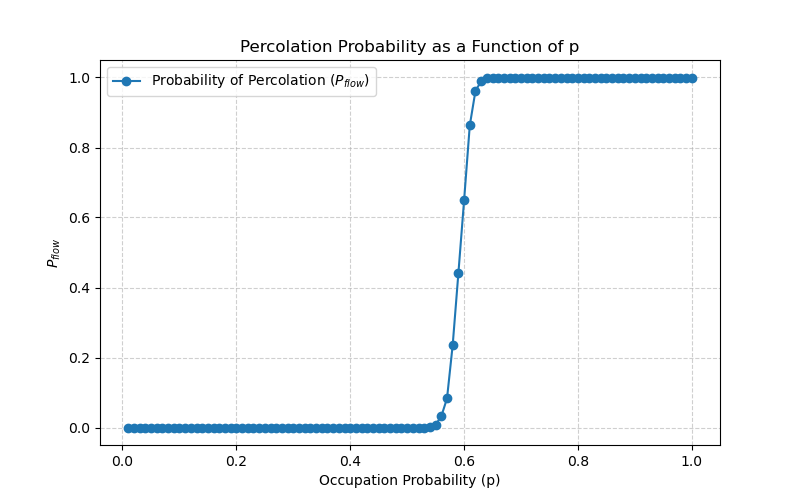
\includegraphics[width=0.9\textwidth]{../PercolationProbability-L100T1000.png}
                \caption{Percolation Probability \( P_{flow} \) vs. \( p \).}
                \label{fig:Pflow}
            \end{figure}

            \item \textbf{Average Maximum Cluster Size:}
            \hfill\break
            Figure \ref{fig:smax} presents the average maximum cluster size \( \langle s_{max} \rangle \) as a function of \( p \).

            \begin{figure}[htbp!]
                \centering
                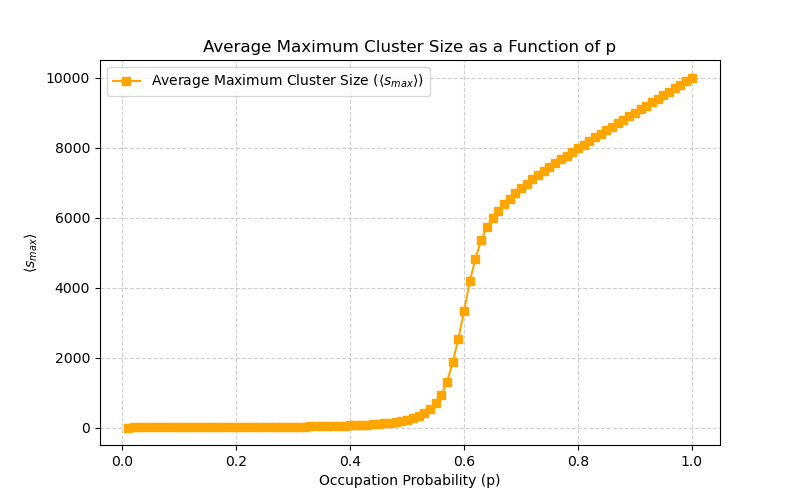
\includegraphics[width=0.9\textwidth]{../AvgMaxCluster-L100T1000.png}
                \caption{Average Maximum Cluster Size \( \langle s_{max} \rangle \) vs. \( p \).}
                \label{fig:smax}
            \end{figure}

            \item \textbf{Cluster Size Distribution:}
            \hfill\break
            The distribution \( n(s, p, L) \) is shown in Figure \ref{fig:ns1000}, illustrating power-law behavior at \( p_c \approx 0.59 \).

            \begin{figure}[htbp!]
                \centering
                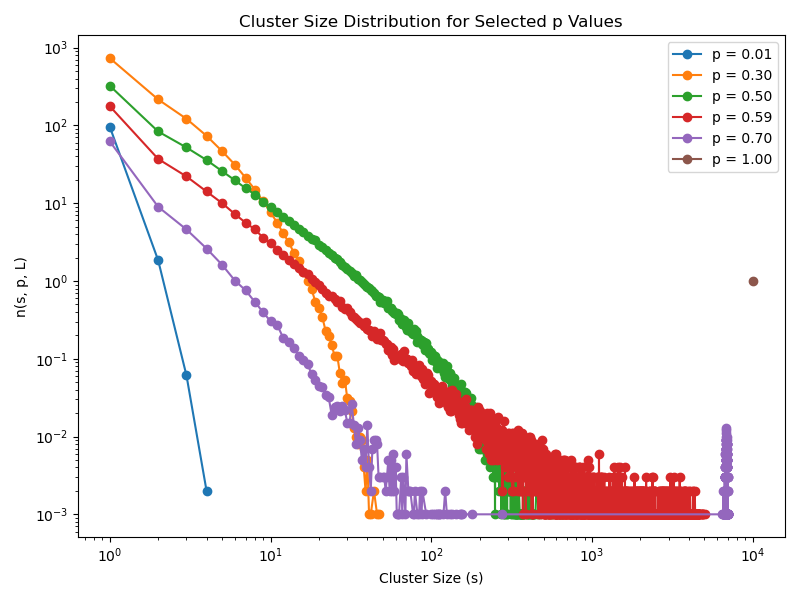
\includegraphics[width=0.8\textwidth]{../ClusterSizeDistribution-L100T1000.png}
                \caption{Cluster Size Distribution \( n(s, p, L) \) for various \( p \) where \( L = 100,\ T = 1000 \).}
                \label{fig:ns1000}
            \end{figure}
            \begin{figure}[htbp!]
                \centering

                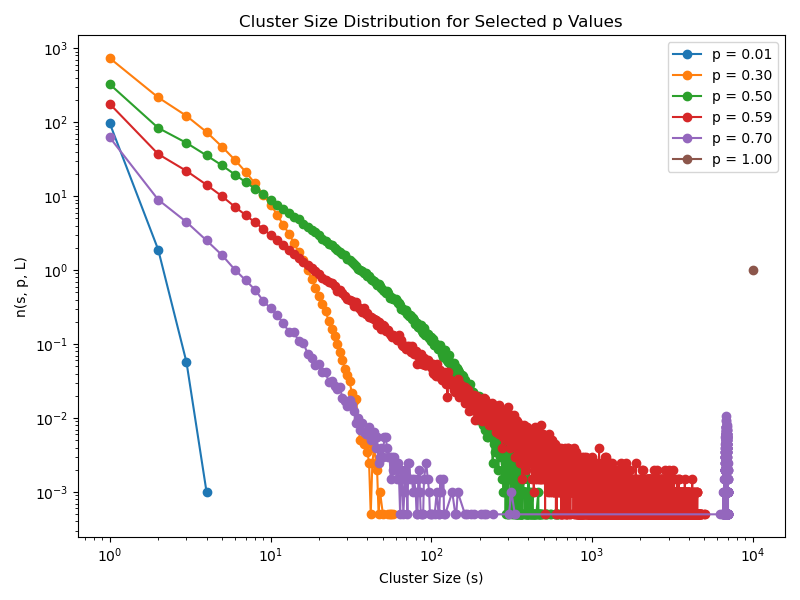
\includegraphics[width=0.8\textwidth]{../ClusterSizeDistribution-L100T2000.png}
                \caption{Cluster Size Distribution \( n(s, p, L) \) for various \( p \) where \( T = 2000 \).}
                \label{fig:ns2000}
            \end{figure}

        \end{enumerate}
        \hfill\break
        \begin{itemize}
            \item Below \( p_c \), the system lacks a spanning cluster, and \( P_{flow} \) is near zero.
            \item Near \( p_c \), \( n(s, p, L) \) exhibits a power-law distribution.
            \item For \( p > p_c \), a spanning cluster dominates, and \( \langle s_{max} \rangle \) increases sharply.
        \end{itemize}

        \hfill\break
        The simulation successfully demonstrates the critical phenomena in percolation. The results align with theoretical predictions, showcasing the percolation threshold and cluster size scaling.


    \end{enumerate}
\end{flushleft}

\end{document}
